\documentclass{article}
\usepackage{kotex, geometry, hyperref, graphicx}

\title{Week 4 - HMI Research Group \\ \large 26 Jun 2017 - 30 Jun 2017}
\author{Long Phi Nguyen (뉀피롱), 한국전자통신연구원}

\begin{document}

  \pagenumbering{gobble}
  \maketitle


  \subsection*{Summary} A fully modular speech program was completed for NAO and can classify/predict user inputs, adding one gesture for NAO to perform as he speaks the text. Data was gathered from NAO's body sensors and converted to feature vectors.

  \subsection*{Points}
  \begin{itemize}
    \item Looked at the NAO API and learned how to use \verb|ALBehaviorManager| to track NAO's behaviors during runtime and \verb|ALMotion| to gather sensor data.
    \item Parsed NAO's motion (see previous point) data to tabulated data involving stiffness, command, and sensor attributes. Converted this data to 5406 feature vectors classified under the 9 groups established in earlier work.
    \item Trained a multilayer perceptron with an average of $80\%+$ accuracy on training data during cross-validation (only 5000 samples).

        \begin{center}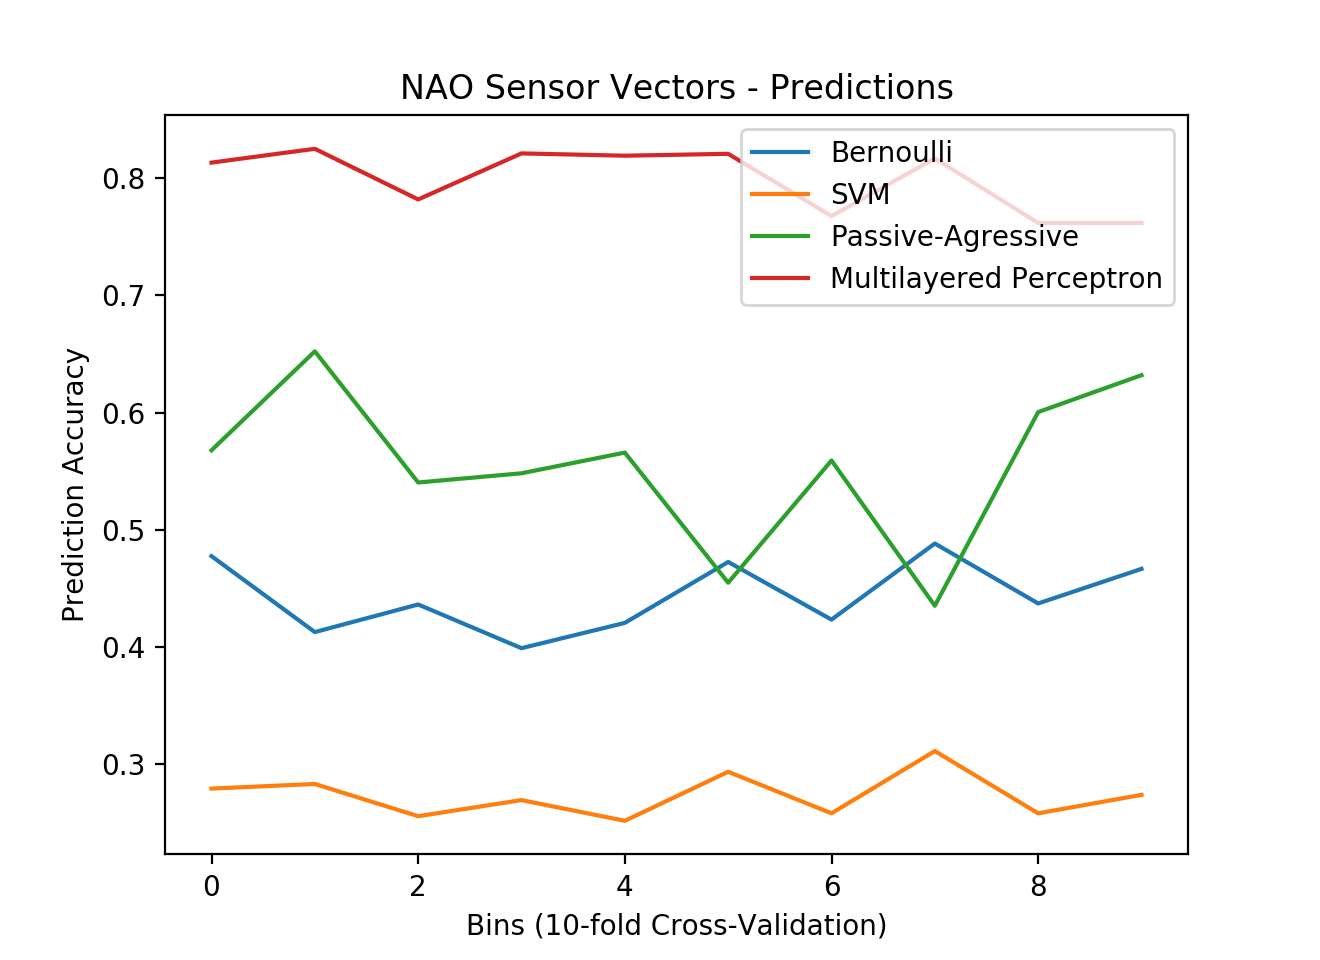
\includegraphics[scale=0.6]{Figure_1.png}\end{center}
    \item Set up Webots and Choregraphe together. Installed 636 behaviors for the simulated NAO---data analysis still supported.
  \end{itemize}

  \subsection*{Plans}
  \begin{itemize}
    \item Find some way to go backwards from the model to generate new movements/gestures that stay true
          to their classifications as NAO speaks.
    \item Learn how to use \verb|ALMotion|'s other functions to manually control NAO's physical movement.
    \item Collect hundreds of thousands of new motion feature vectors from the simulated NAO for more accurate training.
    \item Find any other ways to gather data regarding NAO's sensors and spatial information.
  \end{itemize}

  \subsection*{Addendum}
  All past progress (functions, scripts, etc.) and data made on this project can be found at

  \href{https://github.com/longnguyen1997/nao_animations}{\texttt{https://github.com/longnguyen1997/nao\_animations}}.

\end{document}
